\documentclass[12pt,letterpaper]{article}

\newenvironment{proof}{\noindent{\bf Proof:}}{\qed\bigskip}

\newtheorem{theorem}{Theorem}
\newtheorem{corollary}{Corollary}
\newtheorem{lemma}{Lemma} 
\newtheorem{claim}{Claim}
\newtheorem{fact}{Fact}
\newtheorem{definition}{Definition}
\newtheorem{assumption}{Assumption}
\newtheorem{observation}{Observation}
\newtheorem{example}{Example}
\newcommand{\qed}{\rule{7pt}{7pt}}

\newcommand{\assignment}[4]{
\thispagestyle{plain} 
\newpage
\setcounter{page}{1}
\noindent
\begin{center}
\framebox{ \vbox{ \hbox to 6.28in
{\bf CS578/STAT590: Introduction Machine Learning \hfill #1}
\vspace{4mm}
\hbox to 6.28in
{\hspace{2.5in}\large\mbox{Problem Set #2}}
\vspace{4mm}
\hbox to 6.28in
{{\it Handed Out: #3 \hfill Due: #4}}
}}
\end{center}
}

\newcommand{\solution}[4]{
\thispagestyle{plain} 
\newpage
\setcounter{page}{1}
\noindent
\begin{center}
\framebox{ \vbox{ \hbox to 6.28in
{\bf CS578/STAT590: Introduction to Machine Learning \hfill #4}
\vspace{4mm}
\hbox to 6.28in
{\hspace{2.5in}\large\mbox{Problem Set #3}}
\vspace{4mm}
\hbox to 6.28in
{#1 \hfill {\it Handed In: #2}}
}}
\end{center}
\markright{#1}
}

\newenvironment{algorithm}
{\begin{center}
\begin{tabular}{|l|}
\hline
\begin{minipage}{1in}
\begin{tabbing}
\quad\=\qquad\=\qquad\=\qquad\=\qquad\=\qquad\=\qquad\=\kill}
{\end{tabbing}
\end{minipage} \\
\hline
\end{tabular}
\end{center}}

\def\Comment#1{\textsf{\textsl{$\langle\!\langle$#1\/$\rangle\!\rangle$}}}



\oddsidemargin 0in
\evensidemargin 0in
\textwidth 6.5in
\topmargin -0.5in
\textheight 9.0in

\begin{document}

\solution{Gen Nishida}{\today}{1}{Fall 2014}
% Fill in the above, for example, as follows:
% \solution{John Smith}{\today}{1}{Fall 2014}

\pagestyle{myheadings}  % Leave this command alone

\section{Review Questions}

\begin{enumerate}
\item Assume the probability of getting {\it head} when tossing a coin is $\lambda$.
\begin{itemize}
\item What is the probability of getting the first head at the (k+1)-th toss?
\[
(1-\lambda)^k \lambda
\]
\item What is the expected number of tosses needed to get the first head?\\
Let $k$ be the number of tosses needed to get the first head. Then the expected number of $k$ is defined by
\begin{eqnarray}
E[k]&=&\lambda \times 1 + (1-\lambda) \lambda \times 2 + (1-\lambda)^2 \lambda \times 2 + \cdots\\
(1-\lambda)E[k]&=&(1-\lambda)\lambda + (1-\lambda)^2 \lambda \times 2 + (1-\lambda)^3 \lambda \times 3 + \cdots
\end{eqnarray}
By subtracting (2) from (1), we get
\begin{eqnarray*}
\lambda E[k] &=& \lambda + (1-\lambda) \lambda + (1-\lambda)^2 \lambda + (1-\lambda)^3 \lambda + \cdots\\
 &=&\lambda \frac{1}{1 - (1 - \lambda)}\\
 &=&1 .
\end{eqnarray*}
Thus, $E[k]=1 / \lambda $.
\end{itemize}

\item Let $f(x, y)=3x^2+y^2-xy-11x$

\begin{itemize}
\item What is the partial derivative of $f$ with respect to $x$ $(\frac{\partial f}{\partial x})$? Find $\frac{\partial f}{\partial y}$ as well.
\[
\frac{\partial f}{\partial x}=6x-y-11,\:\:  \frac{\partial f}{\partial y}=2y - x
\]
\item Find a point $(x, y)$ that minimizes $f$.
\[
\left\{
\begin{array}{l}
6x-y-11=0 \\
2y-x=0
\end{array}
\right.
\]
By solving these equations, we get $(x, y)=(2, 1)$.
\end{itemize}

\item 
\begin{itemize}
\item Assume that $\omega \in R^n$ and $b$ is a scalar. A hyperplane in $\mathbb{R}^n$ is the set $\{x : x\in \mathbb{R}^n, \omega^Tx+b=0\}$. For $n=2$ and $n=3$, draw on paper an example of a hyperplane.\\
The hyperplane has it normal vector $\omega$, and it is away from the origin by $-b/\|\omega\|$. The example of a hyperplane for $n=2$ and $n=3$ is in Figure 1.

\begin{figure}[hbtp]
\caption{Figure 1}
\centering
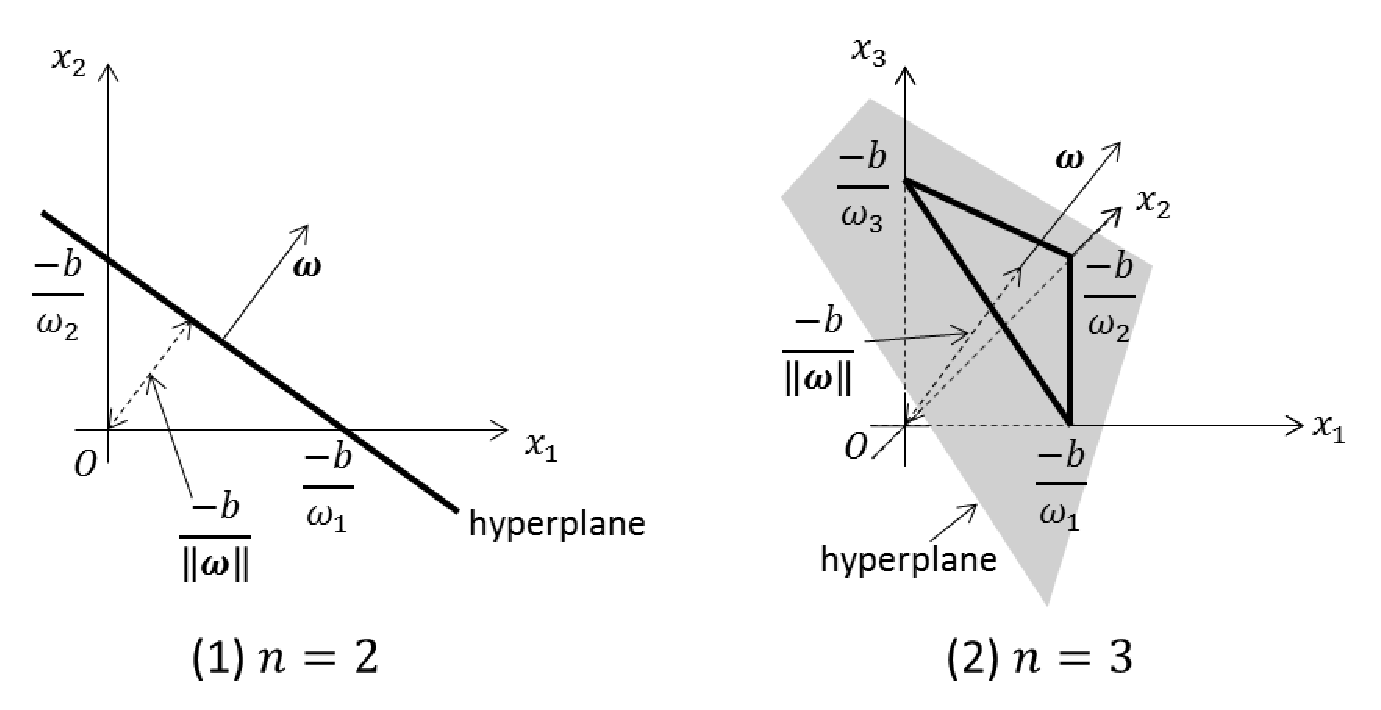
\includegraphics[scale=1]{figure1.eps}
\end{figure}


\item Assume we have two parallel hyperplanes: $\{x: x\in \mathbb{R}^n, \omega^Tx+b_1=0\}$ and $\{x: x\in \mathbb{R}^n, \omega^Tx+b_2=0\}$. What is the distance between these two hyperplanes?
\[
\left|\frac{-b_1}{\|\omega\|}-\frac{-b_2}{\|\omega\|}\right|=\frac{|b_1-b_2|}{\|\omega\|}
\]
\end{itemize}
\end{enumerate}

\section{Basic Concepts}
\begin{enumerate}
\item Define in one sentence: (1) training set, (2) test set, (3) validation set.
\begin{itemize}
\item training set

Training set is a set of data used to optimize a hypothesis function.

\item test set

Test set is a set of real-world data used to measure the accuracy of the hypothesis generated through training and validation phases.

\item validation set

Validation set is a set of data used to estimate the performance of the hypothesis.

\end{itemize}

\item Can you use the validation set as a test set?

No. Since validation set is used to estimate the accuracy of the hypothesis during the validation phase, the resulting hypothesis is optimized for the validation set, and it is meaningless to use the validation set as a test set in order to measure the actual performance for the real-world data.

\item Define in one sentence: overfitting

A hypothesis is said to overfit the training data if it has smaller error on the training data but loses the generalization performance and has larger error on test data.

\item True or False (and why): A learned hypothesis $f$ has a training error $e_{tr}$ and a testing error $e_{ts}$, where $e_{tr} > e_{ts}$.

\begin{itemize}
\item (1) can we say that $f$ overfits to the training data?

False. Since the hypothesis $f$ is optimized for the training data while the test data is unknown during training phase, the training error $e_{tr}$ is smaller than $e_{ts}$ in general, even if $f$ is well generalized. In this case, $e_{tr} > e_{ts}$, which indicates that $f$ is generalized very well.

\item (2) Now, assume that $e_{tr} < e_{ts}$, does $f$ overfit to the training data?

False. Since the hypothesis $f$ is optimized for the training data while the test data is unknown during training phase, the training error $e_{tr}$ is smaller than $e_{ts}$ in general, even if $f$ is well generalized. Therefore, we cannot conclude that $f$ overfits to the training data even if $e_{tr} < e_{ts}$, unless we find another hypothesis $f'$ which has larger error on the training data but smaller error on the test data compared to $f$.

\end{itemize}

\end{enumerate}

\section{Decision Trees}

\begin{enumerate}
\item The "Thrill and Romance" bookstore

\begin{itemize}
\item What is the entropy of the target variable? (Buy)\\
The number of examples labeled "Buy=Y" is 7, while the number of examples labeled "Buy=N" is 4. Thus,
\[
-\frac{7}{11}\log \frac{7}{11}-\frac{4}{11}\log \frac{4}{11}=0.94566
\]

\item What are the attributes considered by the algorithm?\\
All the attributes, "Pages", "Famous Author", "Category", and "Cover Color" should be considered by the algorithm. However, for "Pages", since it is a continuous attribute, we first have to sort examples according to the values of "Pages" and check the mid-point as a possible threshold in order to discretize. The sorted values are as follows:\\
45(-), 50(+), 72(+), 100(-), 120(+), 142(+), 150(+), 200(-), 300(+), 350(+), 1000(-).\\
Thus, the possible thresholds for "Pages" are 47.5, 86, 110, 175, 250, and 675. 

\item What is the first attribute that the algorithm will split the data on? What is its information gain?

The information gain by the split of each attribute is computed as follows.

\begin{itemize}
\item Pages(threshold=47.5)
\begin{eqnarray*}
0.94566 - \left[ 0 \times \frac{1}{11} - \left( -\frac{7}{10} \log \frac{7}{10} - \frac{3}{10} \log \frac{3}{10} \right) \times \frac{10}{11}  \right]\\ = 0.94566 - 0.80117 = 0.14449
\end{eqnarray*}
\item Pages(threshold=86)
\begin{eqnarray*}
0.94566 - \left[ \left( -\frac{2}{3} \log \frac{2}{3} -\frac{1}{3} \log \frac{1}{3} \right) \times \frac{3}{11} + \left( -\frac{5}{8} \log \frac{5}{8} - \frac{3}{8} \log \frac{3}{8} \right) \times \frac{8}{11} \right]\\ = 0.94566 - 0.94458 = 0.00108
\end{eqnarray*}
\item Pages(threshold=110)
\begin{eqnarray*}
0.94566 - \left[ 1.0 \times \frac{4}{11} - \left( -\frac{5}{7} \log \frac{5}{7} - \frac{2}{7} \log \frac{2}{7} \right) \times \frac{7}{11}  \right]\\ = 0.94566 - 0.91289 = 0.03277
\end{eqnarray*}
\item Pages(threshold=175)\\
Same as threshold=110, which is 0.03277.
\item Pages(threshold=250)\\
Same as threshold=86, which is 0.00108.
\item Pages(threshold=675)\\
Same as threshold=47.5, which is 0.14449.
\item Famous Author
\begin{eqnarray*}
0.94566 - \left[ \left( -\frac{5}{7} \log \frac{5}{7} -\frac{2}{7} \log \frac{2}{7} \right) \times \frac{7}{11} + 1.0 \times \frac{4}{11} \right]\\ = 0.94566 - 0.91289 = 0.03277
\end{eqnarray*}
\item Category
\begin{eqnarray*}
0.94566 - \left[ \left( -\frac{4}{5} \log \frac{4}{5} -\frac{1}{5} \log \frac{1}{5} \right) \times \frac{5}{11} + 1.0 \times \frac{6}{11} \right]\\ = 0.94566 - 0.8736 = 0.07206
\end{eqnarray*}
\item Cover Color
\begin{eqnarray*}
0.94566 - \left[ \left( -\frac{6}{9} \log \frac{6}{9} -\frac{3}{9} \log \frac{3}{9} \right) \times \frac{9}{11} + 1.0 \times \frac{2}{11} \right]\\ = 0.94566 - 0.93315 = 0.01251
\end{eqnarray*}
\end{itemize}
The attribute which produces the highest gain is "Pages", so we should use "Pages" as the first attribute to split, and its information gain is 0.14449 if we use threshold=47.5 or 675.
Note that if we split all the values of "Pages", then we will easily be able to separate the labels with information gain = 1.0. However, this will be overfitting, and we do not want to do that.
\item Due to a computer error some of the training examples attributes were deleted! Revise the decision tree training algorithm to deal with missing values in the training data.\\
The goal of training is to minimize the expected loss over the distribution of values of attributes. Intuitively, it is better to use this distribution to estimate the missing values, but, we do not know the distribution in advance. Therefore, the best option would be to assume that the missing values can be all the possible options with equal probability. \\
Suppose the first example in our training data does not have a value of "Famous Author". If we use "Famous Author" as the first attribute to split the tree, then this example contributes a half to both sub-trees. In other words, the subset $S_Y$ for which attribute "Famous Author" has value "Y" will contain 5.5 examples, while the other subset $S_N$ will have 4.5 examples. Also, since the first example is labeled "Buy=Y", in each subset, this example contributes 0.5 to the positive proportion for computing entropy, and the information gain can be computed in the similar manner. In this way, the decision tree training algorithm can deal with missing values in the training data.
\end{itemize}

\item Decision Tree Implementation

\end{enumerate}

\end{document}

